\documentclass{article}

% todo
% forum analysis
  % zotero export quote and reference it in the text
  % make a csv to read the entire forum
  % check a way of analysing into multiple categories

% observable
  % quantify the forum posts by categories, do a sitemap

% Notes
% Citation commands \cite \parencite \textcite 

% Useful packages
\usepackage[a4paper,top=2cm,bottom=2cm,left=3cm,right=3cm,marginparwidth=1.75cm]{geometry}
\usepackage{amsmath}
\usepackage{graphicx}
\graphicspath{{images/}}
\usepackage{svg}
\svgsetup{inkscapelatex=false} % - does not use the latex fonts in imported svg

\usepackage{lmodern}
\usepackage{array}  % Allows for more flexible column formatting
\usepackage{booktabs}  % Improves table aesthetics
\usepackage[skip=0.5ex, justification=raggedright, singlelinecheck=false]{caption}
\usepackage{enumitem}

\PassOptionsToPackage{colorlinks=true, allcolors=blue}{hyperref}
\usepackage[style=apa, backend=biber]{biblatex}

\addbibresource{main.bib}

\newcommand{\getyear}[1]{\citeyear{#1}}

\title{Charting the Beginnings of the Processing Community: Implications for Collaborative Open Source Art Development}
\author{Tibor Udvari}

\begin{document}

\maketitle

\begin{abstract}
What are the dynamics that lead to the creation of a community around a piece of software? How do these dynamics influence the development of the software itself? This thesis explores these questions through the lens of the Processing community, a community of artists and designers who use the Processing software to create interactive art. The paper traces the history of the Processing community from its beginnings in 2001 to the present day, using a combination of interviews, archival research, and analysis of the software development cycle itself. The paper finds that the Processing community was created through a combination of factors, including the software's design, the community's shared values, and the community's shared history. The paper also finds that the community's shared history has influenced the development of the software itself, with the community's values and history influencing the software's design. The paper concludes by discussing the implications of these findings for the development of collaborative open source art software.
\end{abstract}

%\tableofcontents

\section{Introduction}
% \subsection{The Background and Importance of Open Source Projects}
% -- about open source communities in general
% -- importance of open source projects, maybe mention how flash died out, and the recent unity price change ?

\subsection{The Processing Project: A brief overview}
% todo - adapt to focus more on the research question

Processing was developed as a programming language and environment specifically tailored for the media arts communities. Its inception took place at the MIT Media Lab's Aesthetics and Computation Group (ACG) in 2001, led by Ben Fry and Casey Reas. Its foundational concepts build upon the earlier work from the Design By Numbers (DBN) programming platform, a project spearheaded by John Maeda \parencite{fryModernPrometheusHistory2018}.

Ben Fry shed light on the holistic nature of the Processing initiative, noting:
\begin{quote}
"The processing project is a community, a piece of software that you run, and a language. And that order is important."
\end{quote}
\parencite[19:22]{artsatmit2017CASTSymposium2017}

In its design philosophy, Processing introduced the concept of "software sketches". It was designed with an accessible entry point for beginners, while also providing advanced capabilities for experienced users \parencite{reasProcessingProgrammingMedia2006}.

Over the years, Processing has been adopted across various disciplines, showcasing its versatility. To further its impact and development, the Processing Foundation was established, with notable contributors like Daniel Shiffman. The foundation aims to support and expand the reach of the Processing software and its associated projects.

\subsection{Objective and Scope of the Research}
% Choice of processing, because the community has been around for a while and the project is still alive and taught in schools, also at a high school level

% modular toolkit, not a monolith
% community, application, syntax
% commercial software

\section{Literature review}
\subsection{Open Source Contributions: Historical Perspective and Modern Implications}
\subsection{Motivations behind Open Source Contributions}
\subsection{The intersection of Creative Coding and Open Source}
\subsection{Relevant Methodological Approaches in Computer Science and Anthropology}

\section{Methodology}

\subsection{Research Design}
Given the passage of time since the inception of the project, there's potential for memory bias or lack of firsthand experience among contemporary audiences. Research has shown that human memory can be fallible, with biases affecting recall and even leading to the construction of false memories. To mitigate these potential challenges, a quantitative analysis was employed as a vital component of this study.
% todo – find studies referring to these phenomena

However, a comprehensive understanding of the motivations, perceptions, and sentiments of the participants demands more than just quantitative analyses. Anthropological studies have consistently highlighted the limitations of solely relying on numbers to interpret the complex interplay of human experiences, beliefs, and emotions. Thus, interviews stand as a cardinal ethnographic instrument. Engaging in direct dialogues with interlocutors provides access to their lived experiences, emic perspectives, and personal narratives—dimensions that can remain obscured in purely numerical representations. By integrating quantitative methodologies with qualitative ethnographic approaches, this research aspires to achieve a nuanced understanding, addressing both the structural and phenomenological facets of the study's subject.
% todo - simplify this, it's too long and not specific enough

The quantitative research is used to find key contributors to interview.
\subsection{Quantitative Methods}
\subsubsection*{Evolution of Community Discussion Platforms}
In the early days of the Processing project, community interactions predominantly took place on forums. These forums served as a primary channel for users to share experiences, discuss problems, and seek help. Notably, the forum discussions underwent significant transformations in terms of platforms over the years, as can be observed in Table \ref{table:forums}.

\begin{table}[h]
  \raggedright
  \caption{Archival forums composition}
  \label{table:forums}
  \begin{tabular}{l l l c}
      \toprule
      Forum name & Years & URL \\
      \midrule
      Processing alpha forum & 2002-2005 & \href{https://forum.processing.org/alpha/}{forum.processing.org/alpha} \\
      Processing beta forum & 2005-2010 & \href{https://forum.processing.org/beta/}{forum.processing.org/beta}  \\
      Processing 1.0 forum & 2010-2013 & \href{https://forum.processing.org/one/}{forum.processing.org/one} \\
      Processing 2.0 and 3.0 forum & 2013-2018 & \href{https://forum.processing.org/two/}{forum.processing.org/two} \\
      Current processing forum & 2018 - now & \href{https://discourse.processing.org/}{discourse.processing.org} \\
      \bottomrule
  \end{tabular}
\end{table}

\cite{ProcessingForum}

This dynamic shift from one platform to another indicates an evolving user-base and a growing set of needs and tools that community members require for effective collaboration.

\subsubsection*{Shift in Software-Related Discussions}

Initially, software-related discussions were confined to these forums. However, as the project matured, the complexity of issues warranted more specialized platforms for effective tracking and resolution. Consequently, the community transitioned from forums to Bugzilla \parencite{BugzillaArchiveProcessing} and eventually to GitHub Issues\parencite{ProcessingProcessingSource}\parencite{ProcessingProcessing4Processing} . Each shift represented not just a change in platform, but also an evolution in how the community interacted with and contributed to the project. GitHub Issues, for instance, not only enables detailed tracking of software bugs but also allows for more collaborative forms of problem-solving, with capabilities for code reviews, linking pull requests, and so on.

\subsubsection*{The Ecosystem of Libraries}
An important milestone in the Processing ecosystem was the introduction of libraries. These libraries extended the functionalities of the base platform, thereby attracting a broader range of users and contributors. Such an analysis not only sheds light on the diversification of the project but also identifies key contributors and library authors who could potentially be sought out for qualitative interviews. The identification of these contributors adds another layer to our understanding of community participation, opening doors to insights into individual motivations and collective behaviors.

\begin{table}[h]
  \raggedright
  \caption{Data sources}
  \label{table:data-sources}
  \begin{tabular}{l l l c}
      \toprule
      Name & Type & Status \\
      \midrule
      Processing alpha forum & Forum & Parsed \\
      Processing beta forum & Forum & Parsed  \\
      Processing 1.0 forum & Forum & Downloaded \\
      Processing 2.0 and 3.0 forum & Forum  & Not downloaded \\
      Current processing forum & Forum & Not downloaded\\
      Github project & Commit history & Parsed \\
      Processing libraries\textsuperscript{*} & Software release information & Parsed \\
      \bottomrule
      \multicolumn{3}{l}{\footnotesize \textsuperscript{*}Note: The data set was reconstructed from the processing website archive and is not complete.}
  \end{tabular}
\end{table}


\subsubsection{ALPHA Forum Textual Analysis: Approach and Tools}
The research process began by manually reading the forum to identify themes and complemented with quantitative approaches. 
%todo forum composition

% todo
% check how much there is to read, estimate time
% relevance of the topics

\subsubsection{Forum Contributions Descriptive Statistics}

Creating a dataset from the ALPHA forum, which was stated to be the most relevant from Casey.
Creating a dataset from the source control.
Potentially creating and merging datasets from subsequent forums, to coincide with the launch of libraries.

\subsection{Qualitative Methods}
\subsubsection{Interviews: Sample Selection, Interview Guide and Tools}


\section{Data Presentation and Analysis}

\subsection{Quantitative Findings}

\subsubsection{Patterns in Forum Contributions}
There were 11,926 posts across 2,626 topics from 02/08/2002, 15:29 to the 19/04/2005, 09:55 across 1039 authors in the forum.

The alpha forum was a YaBB (Yet another Bulletin Board), it was seperated into forums which conained boards which contained topics which contained posts.

\begin{figure}[h!] 
  \centering 
  \includesvg[pretex=\sffamily\fontsize{5.58pt}{8pt}\selectfont, width=1\textwidth, keepaspectratio]{images/alpha-forums-by-posts.svg}
  \caption{Forums by number of posts}
  \label{fig:forums}  
\end{figure}

\begin{figure}[h!] 
    \centering 
    \includesvg[pretex=\sffamily\fontsize{5.58pt}{8pt}\selectfont, width=1\textwidth, keepaspectratio]{images/figure-alltime-sourcecode-commits.svg}
    \caption{Top 25 source code contributors by number of commits}
    \label{fig:alltime-sourcecode-commits}  
  \end{figure}

\begin{figure}[htbp] 
  \centering
  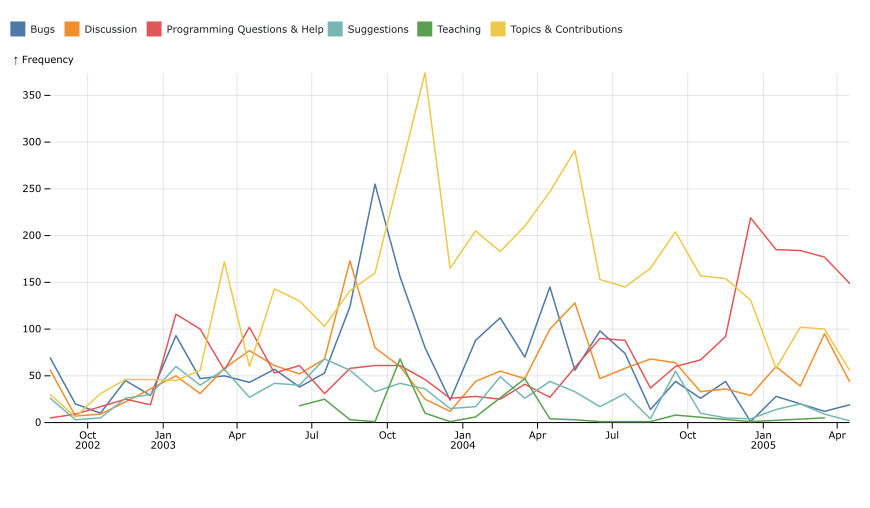
\includegraphics[width=1\textwidth]{alpha-forums-activity.png} 
  % \includesvg[pretex=\sffamily\fontsize{5.58pt}{8pt}\selectfont, width=0.6\textwidth]{images/alpha-forums-activity.svg}
  \caption{Forums activity}
  \label{fig:forum-activity}  
\end{figure}

\subsubsection{Trends in Git Commits}

Considering the \textit{Processing} project, its dependency on its primary contributor, Ben Fry, stands out as a potential vulnerability. Fry's instrumental role over the past two decades underscores the significance of his contributions. Were they to be unexpectedly interrupted, the project could face substantial challenges. This scenario exemplifies a high bus factor risk \parencite{BusFactor2023}, wherein the success and continuity of a project are profoundly dependent on a single, or very few, contributors. Such vulnerabilities appear to be common in open source projects, a sentiment humorously captured in popular culture and comics \parencite{munroeDependency2020}.

\begin{figure}[h!] 
    \centering
    \includegraphics[width=0.75\textwidth]{dependency.png} 
    \caption{Dependency}
    \label{fig:dependency_comic}
    \small Source: \textit{XKCD}, \url{https://xkcd.com/2347/}, licensed under CC BY-NC 2.5.
\end{figure}


\subsection{Qualitative Insights}
\subsubsection{Themes from the ALPHA Forum}
\subsubsection{Interview Highlights and Key Takeaways}

\section{Discussion}

\subsection{Integrating Quantitative and Qualitative Findings}
\subsection{Implications for the Open Source Community}
\subsection{The Unique Case of Processing and Creative Coding}
\subsection{Limitations of the Study}

\section{Conclusion and Recommendations}

\subsection{Recap of Key Findings}
\subsection{Practical Implications for Open Source Projects}
\subsection{Recommendations for Future Research}

\section{Acknowledgements}
I'm grateful to Randall Munroe of XKCD for his insightful and humorous comic strips. The comic "Dependency" from \getyear{munroeDependency2020} is in Figure~\ref{fig:dependency_comic} and cited as~\cite{munroeDependency2020}. It's under the Creative Commons Attribution-NonCommercial 2.5 License (CC BY-NC 2.5). License details: \url{https://creativecommons.org/licenses/by-nc/2.5/}.

\section{Bibliography}
\printbibliography

\section{Appendices}

\subsection{Interview Transcripts}

This is an included file that will be the interview guide
\subsection{Data Collection Tools and Scripts}

\begin{itemize}
    \item \href{https://forum.processing.org/alpha/}{Processing Alpha Forum}
    \item \href{https://observablehq.com/d/042b1cf42ea9bb5e}{Observable Notebook for Forum Analysis}
\end{itemize}


\subsection{List of Forum Threads Analyzed}


\end{document}